% !TEX TS-program = pdflatex
% !TEX encoding = UTF-8 Unicode

% Example of the Memoir class, an alternative to the default LaTeX classes such as article and book, with many added features built into the class itself.

%\documentclass[12pt,a4paper]{memoir} % for a long document
\documentclass[12pt,a4paper,article]{memoir} % for a short document

\usepackage[utf8]{inputenc} % set input encoding to utf8
\usepackage{graphicx} % set input encoding to utf8

% Don't forget to read the Memoir manual: memman.pdf

%%% Examples of Memoir customization
%%% enable, disable or adjust these as desired

%%% PAGE DIMENSIONS
% Set up the paper to be as close as possible to both A4 & letter:
\settrimmedsize{11in}{210mm}{*} % letter = 11in tall; a4 = 210mm wide
\setlength{\trimtop}{0pt}
\setlength{\trimedge}{\stockwidth}
\addtolength{\trimedge}{-\paperwidth}
\settypeblocksize{*}{\lxvchars}{1.618} % we want to the text block to have golden proportionals
\setulmargins{50pt}{*}{*} % 50pt upper margins
\setlrmargins{*}{*}{1.618} % golden ratio again for left/right margins
\setheaderspaces{*}{*}{1.618}
\checkandfixthelayout 
% This is from memman.pdf

%%% \maketitle CUSTOMISATION
% For more than trivial changes, you may as well do it yourself in a titlepage environment
\pretitle{\begin{center}\sffamily\huge\MakeUppercase}
\posttitle{\par\end{center}\vskip 0.5em}

%%% ToC (table of contents) APPEARANCE
\maxtocdepth{subsection} % include subsections
\renewcommand{\cftchapterpagefont}{}
\renewcommand{\cftchapterfont}{}     % no bold!

%%% HEADERS & FOOTERS
\pagestyle{ruled} % try also: empty , plain , headings , ruled , Ruled , companion

%%% CHAPTERS
\chapterstyle{hangnum} % try also: default , section , hangnum , companion , article, demo

\renewcommand{\chaptitlefont}{\Huge\sffamily\raggedright} % set sans serif chapter title font
\renewcommand{\chapnumfont}{\Huge\sffamily\raggedright} % set sans serif chapter number font

%%% SECTIONS
\hangsecnum % hang the section numbers into the margin to match \chapterstyle{hangnum}
\maxsecnumdepth{subsection} % number subsections

\setsecheadstyle{\Large\sffamily\raggedright} % set sans serif section font
\setsubsecheadstyle{\large\sffamily\raggedright} % set sans serif subsection font

%% END Memoir customization

\title{Projet Etamine : Cahier des charges}
\author{Quentin Amelot}
\date{} % Delete this line to display the current date

%%% BEGIN DOCUMENT
\begin{document}

\maketitle
\clearpage
\tableofcontents % the asterisk means that the contents itself isn't put into the ToC

\chapter{Présentation du Projet}

\section{Contexte}
Le projet de développement Etamine est une application multi-structures et multi-tutelles,
développée au laboratoire, qui répond à divers besoins des enseignants chercheurs et
personnels administratifs.
Elle se compose de dizaines de modules répartis dans différents thèmes :
\begin{itemize}
\item administration : gestion des membres, annuaire, trombinoscope… ;
\item outils d’aide à la recherche : gestion de dépôts SVN, GIT, publications, contrats… ; 
\item messagerie : messagerie web, gestion des filtres (antispam, antivirus)… ;
\item … .
 \end{itemize}
Certains modules peuvent utiliser des informations partagées et/ou hébergées en dehors du
laboratoire, accédé de façon anonyme ou authentifiée. Dans le cadre d’Etamine, l’utilisation
des services web est commune.

\section{Objet}
Il s’agit de créer un Web Service qui interagira avec une base de données afin de renvoyer à
des clients des informations sur des pays contenus dans la base de données.
La base de données contiendra diverses informations concernant les pays.
Il faudra aussi créer un client JAVA et un client PHP afin de communiquer avec le Web Service.
Ces clients ne requerront pas d’authentification pour utiliser le Web Service. Le client PHP
pourra être intégré dans un navigateur et le client JAVA permettra de s’assurer une intégration
dans des applications.
Nous créerons aussi une application de gestion afin d’effectuer des modifications sur la base
de données.
Ce client possédera un système d’authentification afin que seuls les utilisateurs autorisés
puissent modifier la base.

\section{Organisation}
Six personnes doivent réaliser ce projet :
\begin{itemize}
\item Le chef de projet : Quentin AMELOT
\item Le responsable recherche et développement : Damien LARMINÉ
\item Le responsable d’assurance qualité (QA) : Paul BAUDOUIN
\item Le responsable de la documentation : Jérémie NIZOU
\item Le développeur PHP : Gisio TABERA
\item Le développeur JAVA : Fayize KAIMOU
\end{itemize}
Chaque personne possède un rôle bien précis dans la réalisation de ce projet, chaque personne
est donc un maillon important de la chaîne.

\section{Environnement}
L'application sera réalisée en Java SE 1.7 à l'aide de l’IDE NetBeans ainsi que la plateforme
SVN, car l'application devra s'installer sur n'importe quel type de machines.
Nous aurons besoin notamment des librairies Hibernate (à confirmer) pour la synchronisation
avec la base de données. Le choix du Framework pour l’interaction avec la base de données se
fera plus tard dans le développement du projet.
Nous utiliserons jUnit ainsi que Concordion pour les différents tests unitaires et fonctionnels.
En ce qui concerne la base de données et le développement PHP, nous utiliserons
phpMyAdmin et son équivalent Mac.
Nous utiliserons également l’architecture REST (Representational State Transfer), c’est un
style d’architecture permettant de construire des applications pour Web-Service, Web,
intranet. Ce n’est pas une technologie à part entière, mais un ensemble de conventions et de
bonnes pratiques à respecter. Il utilise les spécifications originelles du protocole HTTP.
Nous utiliserons REST pour ne pas réinventer une surcouche comme le font XML-RPC ou
SOAP.

\section{Outils complémentaires}
Nous utiliserons l’application web TRAC. Son objectif est de simplifier le suivi et le
traitement efficace des problèmes de logiciel, améliorations et les progrès d’ensemble. Cela
nous permettra de faciliter la gestion du projet.
Un wiki sera mis à disposition afin de répondre aux questions les plus évidentes. Cependant,
pour des demandes plus poussées, il sera nécessaire de prendre contact avec l’équipe de
développement.

\chapter{Objectifs}

\section{Points clés sur les besoins fonctionnels}
Plusieurs points clés sont nécessaires pour bien répondre aux attentes. Premièrement, il s'agit
de rendre l'application exécutable sur un réseau local. Il faut qu'il soit facile d’installation et
d'utilisation sur n'importe quel type de machines, c'est-à-dire sur un maximum de systèmes
d'exploitation, type Linux, Windows ou Mac.
Un guide d'utilisation ainsi qu’un guide d’installation seront fournis.

\section{Limites du projet}
Le projet n’a pas de limites : il est censé être diffusé au grand public. Un budget n'est pas
nécessaire, car nous n’utiliserons que des logiciels libres et l'utilisation de licences n'est pas
obligatoire pour réaliser correctement notre projet.
Pour que le projet ait une plus grande envergure, la solution serait de le rendre disponible en
ligne, donc accessible pour n'importe qui, peu importe l'endroit.
Le manuel d’utilisation pourra être traduit ou directement rédigé en anglais pour une
meilleure compréhension par le grand public.

\chapter{Spécifications}

\section{Base de données}
La base de données doit servir de référentiel pour les pays.
\break
Le référentiel des pays sera accessible à distance, pour chaque pays sera disponible :
\begin{itemize}
\item le libellé
\item le code ISO
\item la devise
\item les coordonnées
\item le risque
\item la nationalité
\item le nom du pays en français
\item le nom du pays en anglais
\item la valeur per diem
\item le taux de change
\end{itemize}
Ce référentiel sera donc accessible via le biais d’un Web Service.

\underline{La structure de la table :}
\begin{center}
\begin{tabular}{|| l | l ||}
	\hline
	Nom & Type \\
	\hline \hline
	ID & int(11) \\
	\hline
	indicatif & varchar(10) \\
	\hline
	nationalité & varcahr(100) \\
	\hline
	nom\_EN & varchar(100) \\
	\hline
	nom\_FR & varchar(100) \\
	\hline
	monnaie\_code & varchar(5) \\
	\hline
	monnaie\_perdiem & decimal(10,4) \\
	\hline
	taux\_change & decimal(10,7) \\
	\hline
	coords1 & text \\
	\hline
	coords2 & text \\
	\hline
	coords3 & text \\
	\hline
	coords4 & text \\
	\hline
	coords5 & text \\
	\hline
\end{tabular}
\end{center}

\break

\underline{Le dictonnaire de données :} \break
\begin{tabular}{|| l | l | l ||}
	\hline
	Champ & Descriptif & Remarque\\
	\hline \hline
	ID & identifiant & Clé primaire de la base de données \\
	\hline
	indicatif & code ISO & Code sur 2 ou 3 lettres du pays \\
 	\hline
	nationalité & nationalité du pays &  Ex : France=Française, etc. \\
	\hline
	nom\_EN & nom du pays en anglais &  \\
	\hline
	nom\_FR & nom du pays en français &  \\
	\hline
	monnaie\_code & code de la monnaie & Ex : Euro=EUR, Royaume-Uni=GBP \\
	\hline
	 monnaie\_perdiem & montant de la monnaie per diem & \parbox{10cm}{L’argent attribué par jour pour \\ vivre dans ce pays} \\
	\hline
	 taux\_change & taux de change&  Par rapport à l’Euro\\
	\hline
	 danger & symbole du danger du pays  & \parbox{10cm}{ 0 si pas dangereux, 1 si dangereux  \\ Risque etabli par le gouvernement} \\
	\hline
	 coords1 & & \parbox{10cm}{Coordonnées du pays, \\ utilisé pour la carte interactive}\\
	\hline
	 coords2 & & \\
	\hline
	 coords3 & & \\
	\hline
	coords4 & &  \\
	\hline
	coords5 & & \\
	\hline
\end{tabular}
\break \break

Exemple des données contenues :
\break
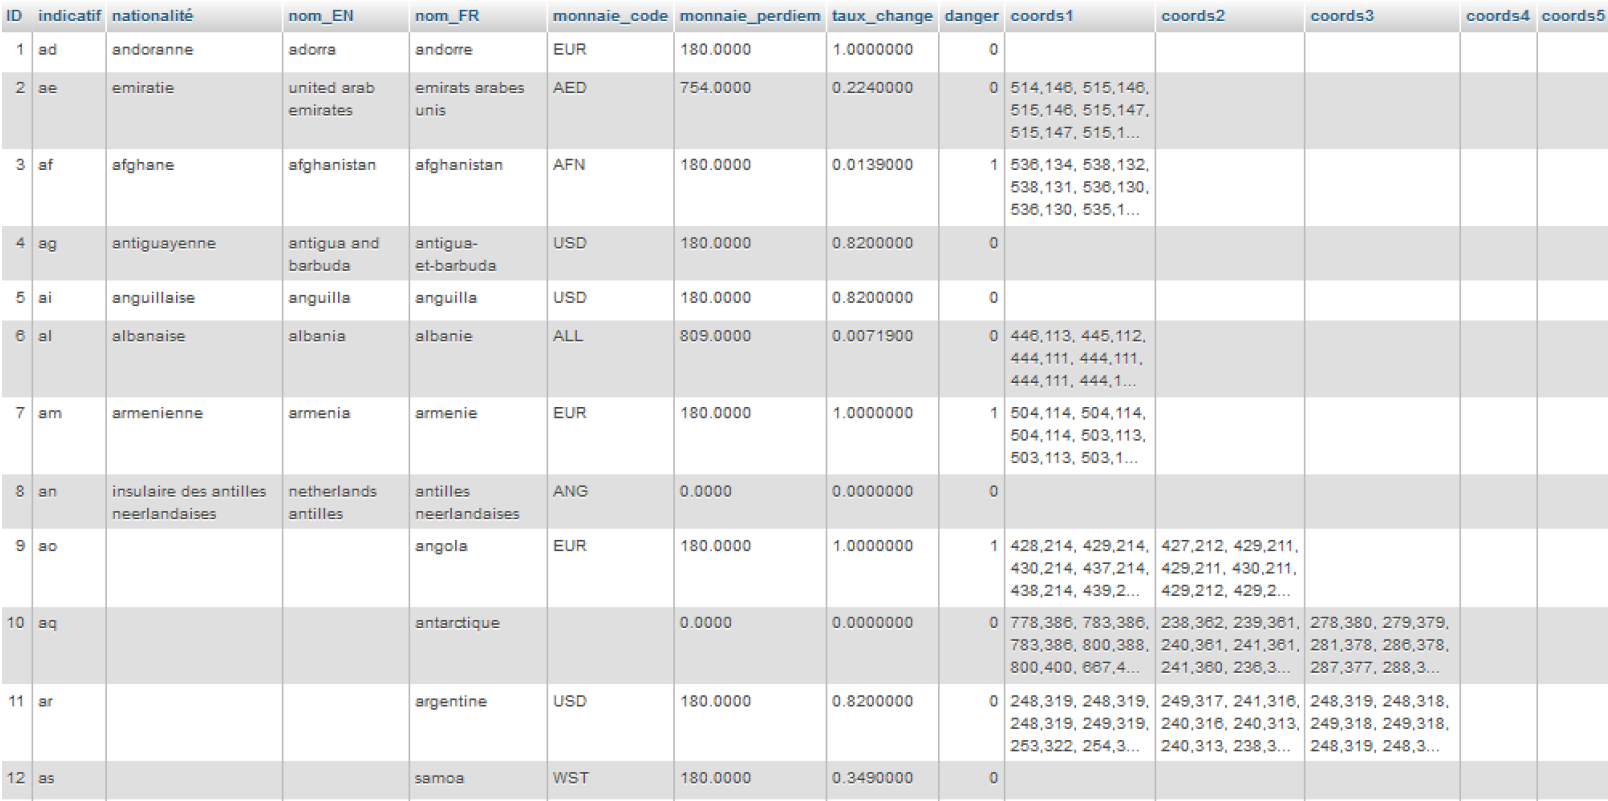
\includegraphics[scale = 0.4]{images/Image1}


\section{Web Service}
Le serveur permettra la récupération des données depuis la base de données. Elles seront
transmises aux clients.
Ce serveur est une application JAVA ne comportant pas d’interface graphique (GUI), mais
regroupant différentes méthodes pour accéder aux données et les renvoyer. Parmi ces
méthodes, nous trouverons :
\begin{itemize}
\item envoyerDonnées()
\item recevoirRequete()
\item pays()
\item paysParNom()
\item paysParRisque()
\item paysPar[...]()
\item …
\end{itemize}

Ceci est une liste non exhaustive permettant de saisir les principales interactions possibles
avec ce serveur.

\section{Clients Web Service}
Les clients PHP et JAVA seront conçus avec les mêmes fonctionna lités de base.
Ils exécuteront des requêtes prédéfinies choisies par l’utilisateur.
Les utilisateurs des clients du Web Service n’ont pas besoin d’être authentifiés pour accéder
aux données.
Les captures d’écran suivantes donnent une idée des fonctionnalités des clients.
L’utilisateur effectue une requête via un formulaire :
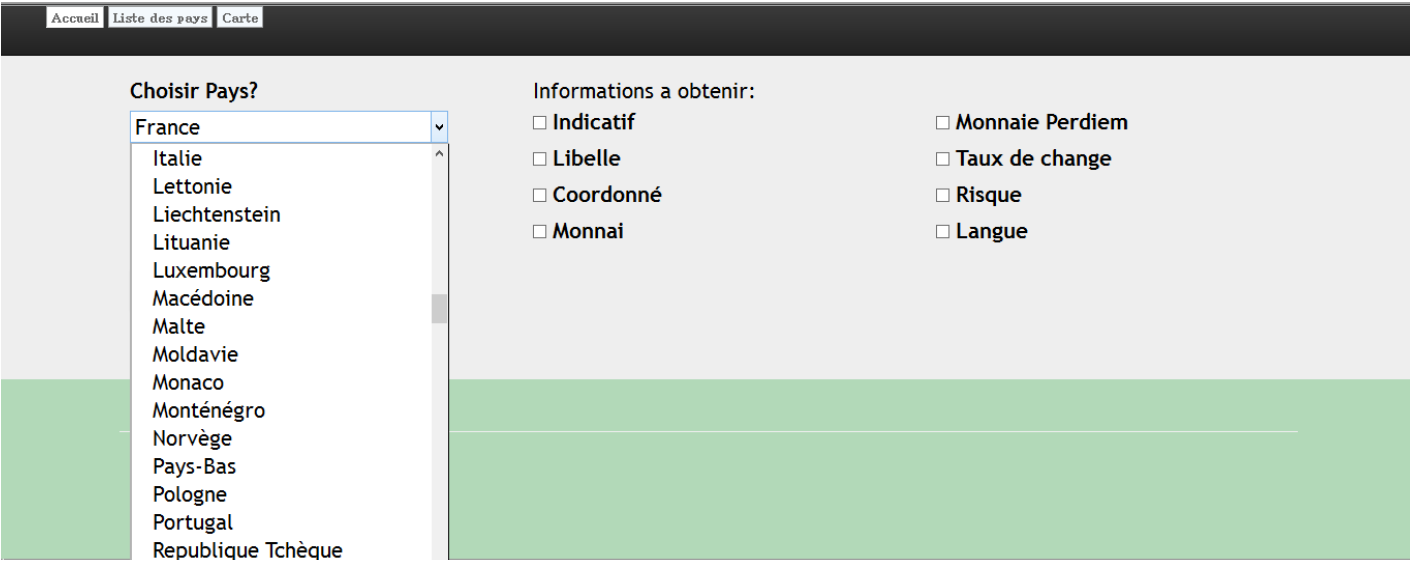
\includegraphics[scale = 0.4]{images/Image2}
L’utilisateur consulte la liste des pays, disponible à tout moment :
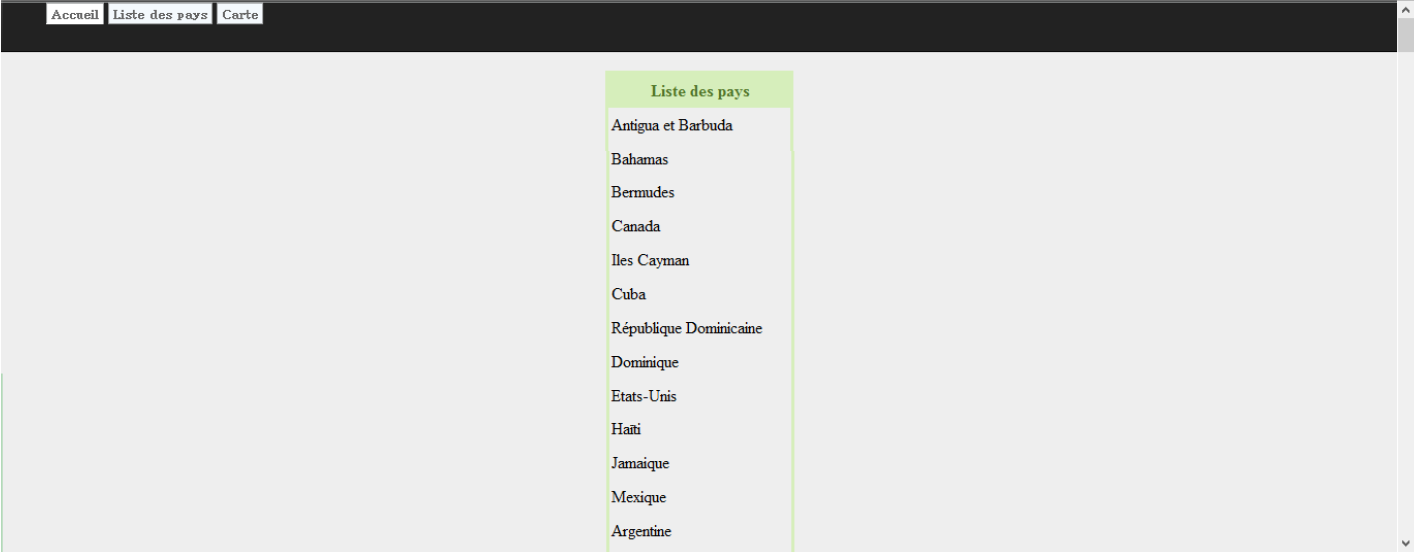
\includegraphics[scale = 0.4]{images/Image3}
L’utilisateur consulte une carte interactive des pays :
\break
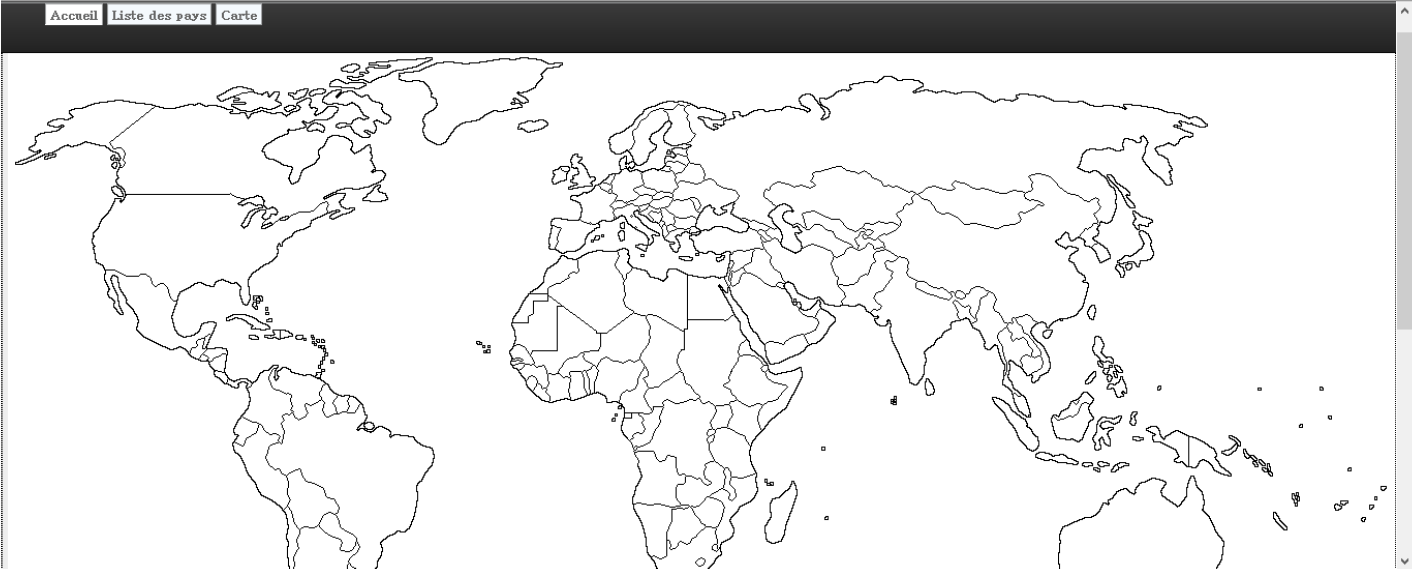
\includegraphics[scale = 0.4]{images/Image4}
En passant sur un pays avec la souris, le pays sera colorié et un type d’information choisi sera
affiché, par exemple la devise ou le nom du pays.

\section{Application de gestion}
L’application de gestion offrira quant à elle la possibilité à l’administrateur de modifier sa base
de données facilement, avec un certain nombre d’actions de maintenances prédéfinies :
\begin{itemize}
\item Ajouter un pays
\item Modifier un pays
\item Supprimer un pays
\item Consulter la base de données
\end{itemize}
Ces actions ne seront disponibles qu’après s’être authentifié sur une page :
Unefois l’utilisateur connecté, il pourra interagir avec la base de données via une interface
avec des boutons pour choisir les actions (ajouter un pays, modifier un pays, etc.) puis via des
formulaires pour préciser les données à ajouter ou à changer.


\includegraphics[scale = 0.4]{images/Image5}
\break \break
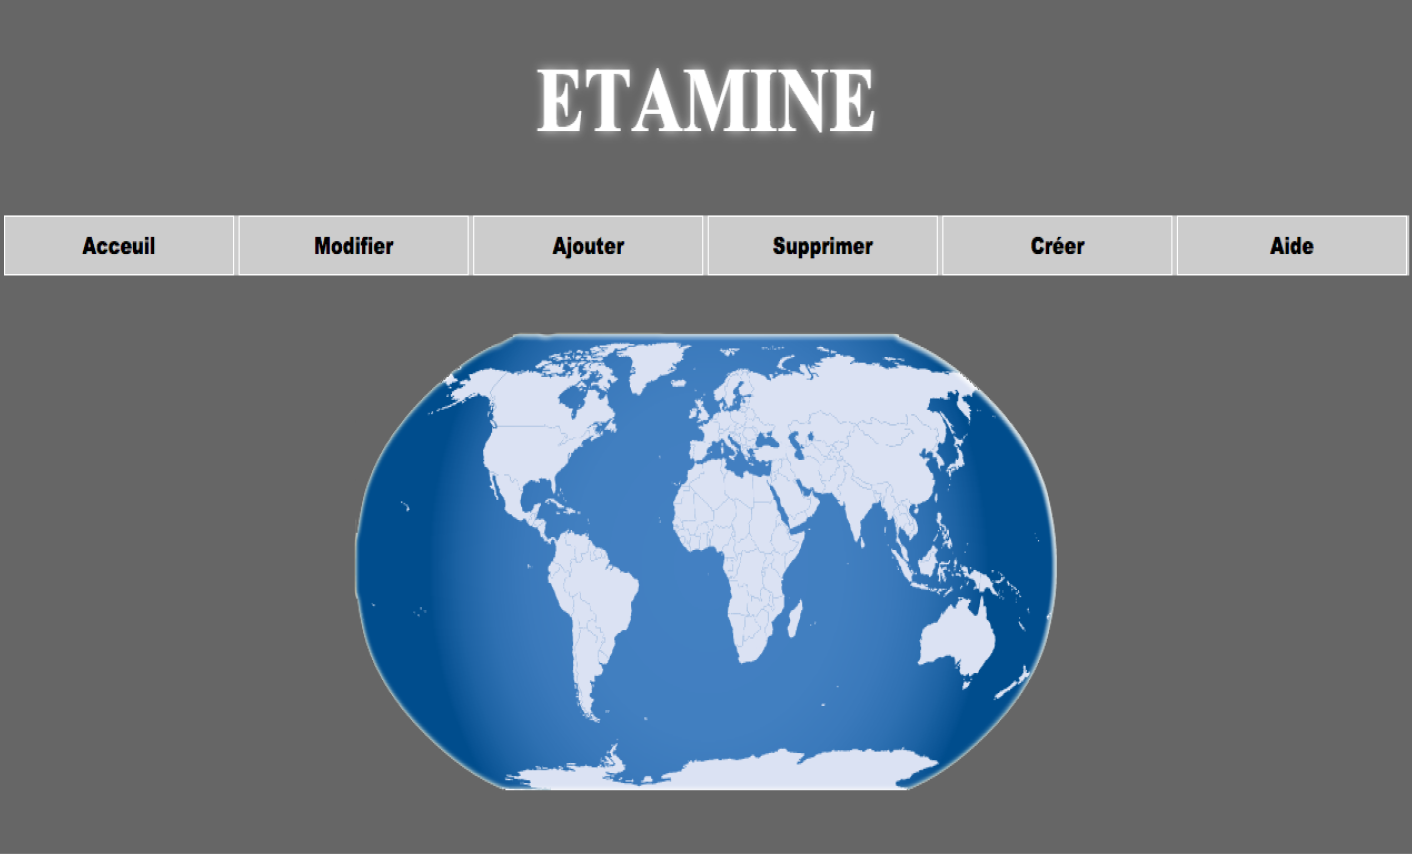
\includegraphics[scale = 0.4]{images/Image6}
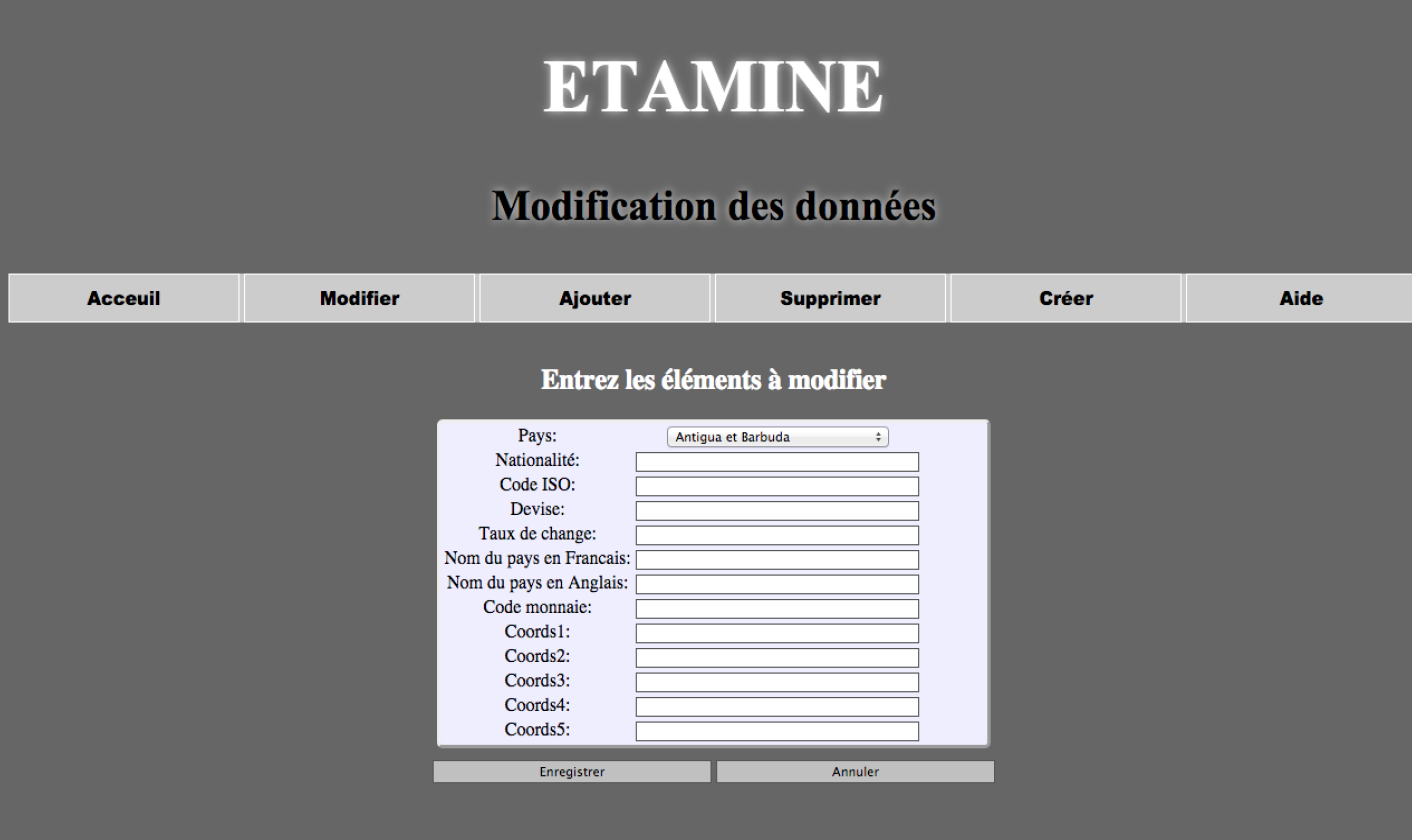
\includegraphics[scale = 0.4]{images/Image7}

\chapter{Livrables}

\section{Documents à remettre}
\begin{itemize}
\item Cahier des charges : Document contenant toutes les spécifications du projet ainsi que
son organisation et le calendrier qui le régit
\item Documentation d’installation : Document contenant les protocoles utilisés pour
installer tous les programmes fournis
\item Document utilisateur : Document contenant l’utilisation des programmes fournis ainsi
que l’explication du code pour faciliter la réintégration
\item Rapport de projet : Document expliquant le travail fourni, et le fonctionnement du
groupe durant la période de développement
\end{itemize}

\section{Programmes à remettre}
\begin{itemize}
\item La base de données :
C’est le référentiel des pays contenant toutes les informations relatives aux pays
\item Le serveur de Web Service en JAVA
C’est l’application (le web service) qui permet la communication avec la base de données
\item Le client PHP
Un client destiné essentiellement à l’intégration dans des sites web.
\item Le client JAVA
Ce client est destiné à l’intégration dans des applications.
Les sources des deux clients seront disponibles, afin de faciliter la réintégration dans de
futures applications. Le code devra être commenté et clair.
\item Le Client de gestion
Destiné à la gestion, il sera privé et réservé à l’administration de la base de données. Il
comportera une interface graphique simple permettant à des utilisateurs non familiers avec
SQL de modifier la base de données.
\end{itemize}

\chapter{Calendrier}

\section{Date de fin de projet}
Les dates de soutenances ne nous ont pas encore été communiquées, il semblerait que le
projet soit évalué fin avril.
Il est impératif que le projet soit terminé la semaine du 20 avril 2014 au plus tard, pour
permettre au client de bien prendre en main l'application. Afin qu'il puisse le jour de la
soutenance suivre correctement notre présentation.

\section{Échéances intermédiaires}
Chaque séance permettra à l'équipe de faire le point sur les différentes avancé de chaque rôle
dans la
réalisation du projet.
Un contact constant par mail sera maintenu avec le client pour éviter tout phénomène de
tunnel, et de pouvoir, éventuellement, réorienter le projet.

\section{Diagramme de GANTT}
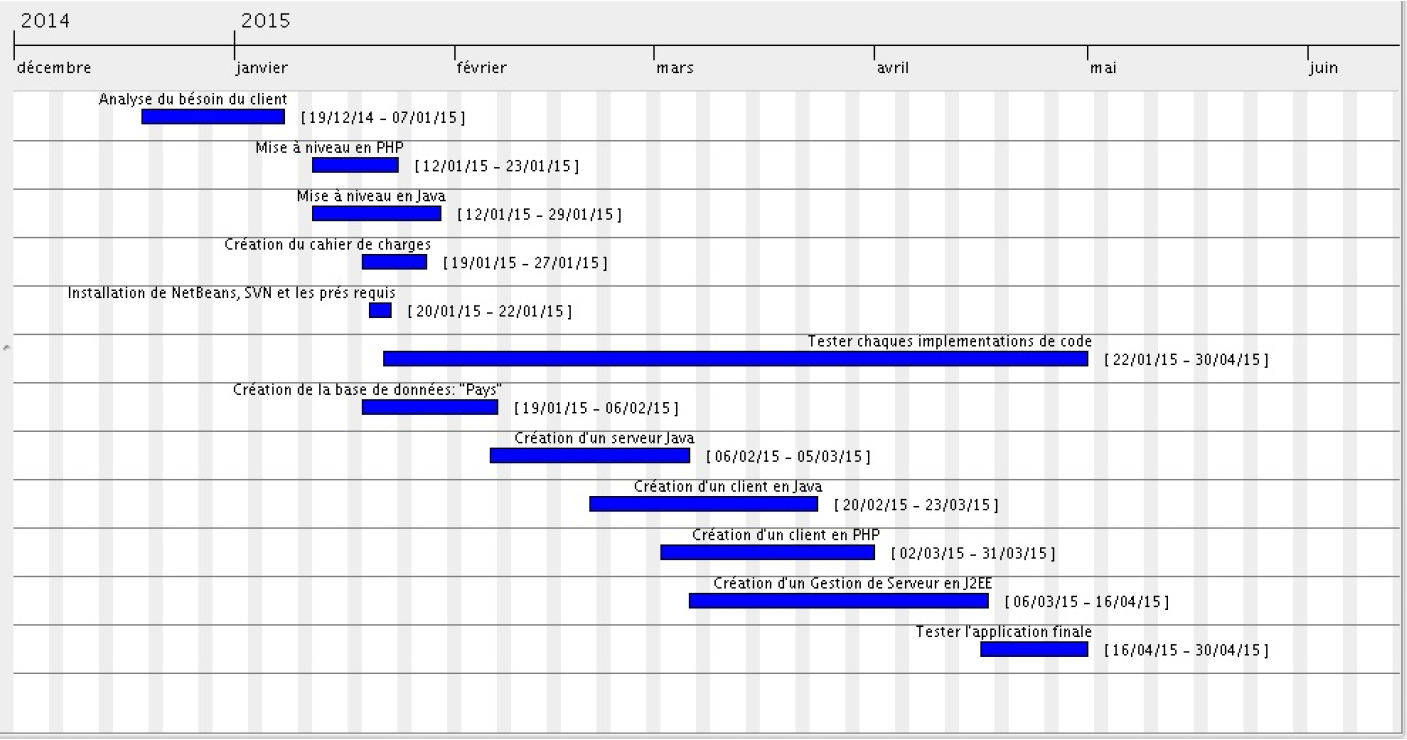
\includegraphics[scale = 0.4]{images/Image8}
\end{document}
